\documentclass[11pt]{article}
\usepackage[top=30truemm,bottom=30truemm,left=25truemm,right=25truemm]{geometry}
\usepackage[dvipdfmx]{graphicx}
\usepackage{float}
\begin{document}
\title{金蒸着の条件}
\author{平松}
\maketitle

\abstract
金薄膜の蒸着条件と結晶特性の関係について先行論文をまとめる。

\section{蒸着}
\subsection{基盤}
\begin{enumerate}
\item {\bf LiF基盤上に金をスパッタリング(レート0.22 nm/s)で80nm成長させたとき、Elipsometryで測定した誘電率(波長200nm-1700nm)は金単結晶のものとよく一致した。またその後550度でアニーリングしても結晶特性にほぼ影響を与えなかった。}\\ フッ化リチウム(LiF)は金と同じ面心立方構造をもち、格子定数のミスマッチが1.5\%以下。したがって界面エネルギーが低く金のエピタキシャル成長が可能。
\cite{Au_on_LiF}\\

\item  {\bf $CaF_2, mica, Si$の基盤上に室温で金薄膜を80nm熱蒸着させると、それぞれ15,20,25nmオーダーの球形の結晶粒が得られた。}\\これはイオン相互作用(ionic interaction)とそれに起因するmigration lengthの違いで理解できる。十分に蒸着速度が遅ければ、表面粗さは膜の厚さの平方根に比例したパラメータのポアソン分布でモデル化できる。\cite{Au_mica_glass_etc}\\

\item  {\bf 電子ビーム蒸着法をもちいて、Ni/Geを~2nm、その上に銀を50nm成長させると、Ni上でプラズモニック特性の改善が見られた。} \cite{Ag_on_Ni_Ge}\\
\begin{figure}[H]
\centering
  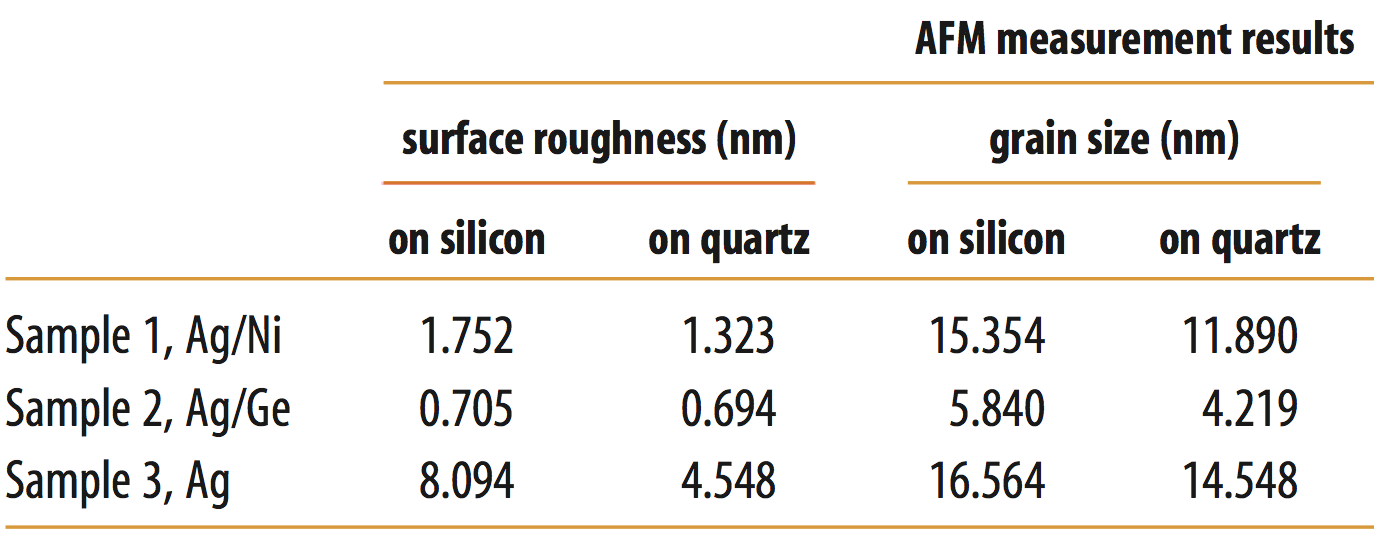
\includegraphics[width=7cm]{./Ag_on_Ni_Ge}
\end{figure}

\item  {\bf ガラス基板上に中間接着層をはさんで作成した金ナノアンテナの光散乱強度が中間接着層の材質に依存する}\\ 中間接着層の厚さ-2nm、金薄膜厚さ-17nm\\The increased dephasing rate is explained in terms of the dissipative dielectric function of the Ti and chemical interface damping where the conduction electrons are transferred across the metal-metal interface.\cite{Au_on_Ti}\\
\begin{figure}[H]
\centering
  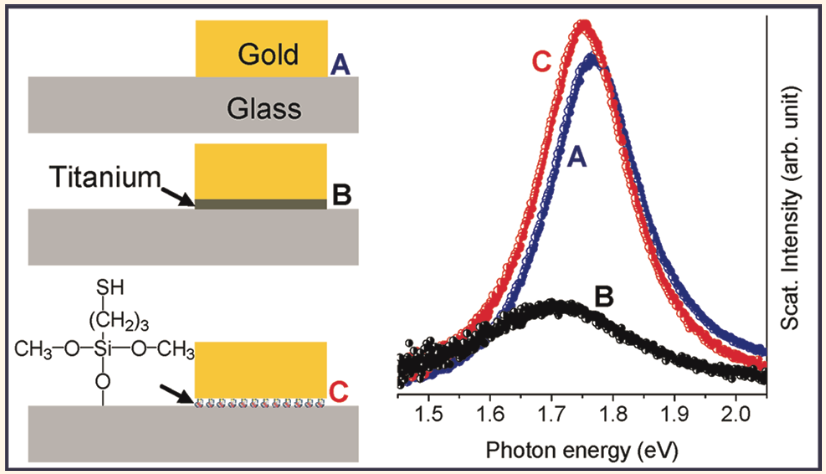
\includegraphics[width=7cm]{./Au_on_Ti}
\end{figure}


\item そのほかにも過去の誘電率測定を追試して、なぜ計測値が一致しないのか基盤の材質などの観点から考察した論文がある\cite{Au_on_Ti_Ali}

\item また高品質窒化ガリウム結晶を成長させるために開発された、低温バッファ層技術も参考にしたい。
\end{enumerate}

\subsection{蒸着レート}
蒸着レートを上げると結晶粒の大きさは大きくなるが、その大きさのバラつきも大きくなる\cite{Deposition_rate}

\subsection{膜厚}
膜を厚くすると結晶粒の大きさは大きくなる\cite{Thickness_dependence}

\subsection{蒸着時の温度}
平均粒径と表面粗さは蒸着時の温度が高くなるにつれて大きくなる(熱蒸着)\\ enhancing the desorption of adsorbed surface contaminants, lowering supersaturation thus allowing the dilute gas of adatoms sufficient time to reach the equilibrium positions, providing activation energy of adatoms to occupy the positions of potential minima, enhancing recrystallization due to the coalescence of islands by increasing surface and volume diffusion and assisting a possible ionization of surface atoms.)  \cite{Au_mica_glass_etc}

\section{アニーリング}
アニーリングを行うと微細構造の変形があることが報告されている\cite{Anneal_antennas}\cite{Anneal_MIR_grating} 。そこで解決策として、金属(金)でつくった構造の周りをHydrogen silsesquioxaneで囲み、アニール後フッ(化水素)酸で溶かすという方法が提案されている。\cite{Encapsulated_Annealing}

\section{結晶粒の大きさの評価方法}
結晶粒の大きさだけでなく、その大きさの分布も推定できることが望ましい。\\
crystallographic grain sizes, Morphological grain sizesというものがあるらしい。

\subsection{AFM}
\subsubsection{手作業で推定}
よく使われている。

\subsubsection{correlation function}
\cite{Ag_on_Ni_Ge}

\subsection{Xray Diffraction}
一般的。結晶粒の平均の大きさしか測れない。

\section*{付録:主要な金属の格子定数}

\begin{itemize}
\item 14 Silicon \\
543.09, 543.09, 543.09 pm
\item  22 Titanium \\
 295.08, 295.08, 468.55 pm
\item  24 Chromium\\
 291., 291., 291. pm
\item  25 Manganese\\
 891.25, 891.25, 891.25 pm
\item  28 Nickel\\
 352.4, 352.4, 352.4 pm
\item  29 Copper\\
 361.49, 361.49, 361.49 pm
\item  30 Zinc\\
 266.49, 266.49, 494.68 pm
\item  32 Germanium\\
 565.75, 565.75, 565.75 pm
\item  47 Silver\\
 408.53, 408.53, 408.53 pm
\item  79 Gold\\
 407.82, 407.82, 407.82 pm 
\item Quartz \\
 491.27, 491.34 pm 
\end {itemize}
出典: http://www.periodictable.com/Elements/025/data.html

\bibliographystyle{unsrt}
\bibliography{../Reference}

\end{document}
